Neste capítulo serão apresentados e analisados os resultados da simulação de um incêndio florestal, em quatro cenários distintos.
Estes cenários apresentam configurações de modelo semelhantes, diferindo apenas nos seguintes parâmetros: velocidade do vento no sentido norte e este, e inclinação do terreno.
Todos os valores podem ser consultados na Tab.~\ref{tab:scenarios}.

\begin{table}[tbhp]
    \centering
    \begin{tabular}{c|cccc}
        \hline
        \textbf{Propriedades} & \textbf{Cenário 1}        & \textbf{Cenário 2} & \textbf{Cenário 3} & \textbf{Cenário 4} \\
        \hline
        Densidade             & 25\%                      & -                  & -                  & -                  \\
        Carvalhos/pinheiros   & 271/272                   & -                  & -                  & -                  \\
        Prob.\ propagação     & 0.4                       & -                  & -                  & -                  \\
        Temperatura inicial   & $\SI{20}{\degreeCelsius}$ & -                  & -                  & -                  \\
        Inclinação & \ang{30}                  & \ang{-30}          & \ang{30}           & \ang{-30}          \\
        Vento Norte           & -10                       & -10                & 10                 & 10                 \\
        Vento Este            & 15                        & 15                 & 15 & 15                 \\
        \hline
    \end{tabular}
    \caption{Configurações dos diferentes cenários}
    \label{tab:scenarios}
\end{table}

Cada cenário foi executado onze vezes, e para cada execução foram com guardados em CSV os seguintes parâmetros do modelo: tick, número de árvores ardidas - absoluto, percentual e para cada tipo de árvore, número de fagulhas na floresta, temperatura média e máxima.


\section{Cenário 1}\label{sec:scenario1}

O primeiro cenário apresenta uma inclinação positiva do terreno, de \ang{30}, com vento sudeste de intensidade $(-10, 15)$ \si{\meter\per\second}, ou seja, a favor da propagação do incêndio.
O modelo terminou com 71.3\% da floresta ardida, após 3377 ticks, ou 387 árvores em termos absolutos - 205 carvalhos e 182 pinheiros.

De início, o fogo propaga-se rápido, como se pode notar pelas curvas acentuadas das Fig.~\ref{fig:S1ForestBurnt} e~\ref{fig:S1TreesBurnt}, acabando por abrandar por volta dos 2000 ticks e estabilizar pouco tempo depois.
As fagulhas, dado a sua aleatoriedade e condições específicas de geração, apresentam uma evolução mais errática, evidente pela Fig.~\ref{fig:S1Sparks}, só começando a espalhar-se a partir dos 400 ticks, e atingindo um pico de 15 fagulhas por tick por volta dos 1500 ticks.
Dado que a floresta é pouco densa, a temperatura média não ultrapassou os $\SI{330}{\degreeCelsius}$, já a temperatura máxima, atingida após 800 ticks (Fig.~\ref{fig:S1Temp}), foi muito superior, cerca de $\SI{1870}{\degreeCelsius}$.

\begin{figure}[H]
    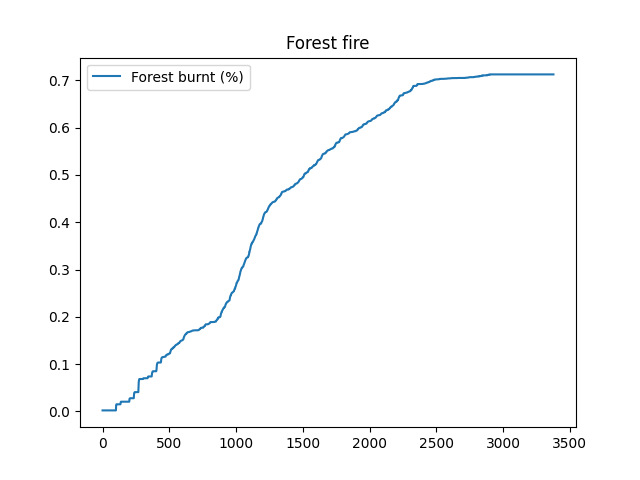
\includegraphics[width=\linewidth]{../src/runs/scenario1/forest_fire}
    \caption{Cenário 1 - Total de floresta ardida (em percentagem)}
    \label{fig:S1ForestBurnt}
\end{figure}

\begin{figure}[H]
    \centering
    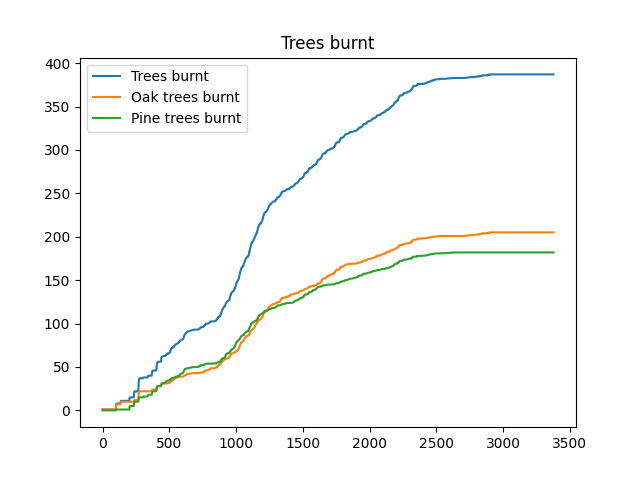
\includegraphics[width=\linewidth]{../src/runs/scenario1/trees_burnt}
    \caption{Cenário 1 - Total de árvores ardidas}
    \label{fig:S1TreesBurnt}
\end{figure}

\begin{figure}[H]
    \centering
    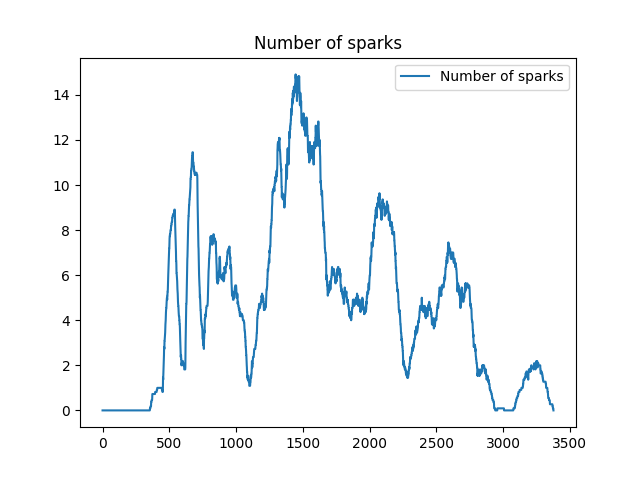
\includegraphics[width=\textwidth]{../src/runs/scenario1/sparks}
    \caption{Cenário 1 - Evolução do número de fagulhas}
    \label{fig:S1Sparks}
\end{figure}

\begin{figure}[H]
    \centering
    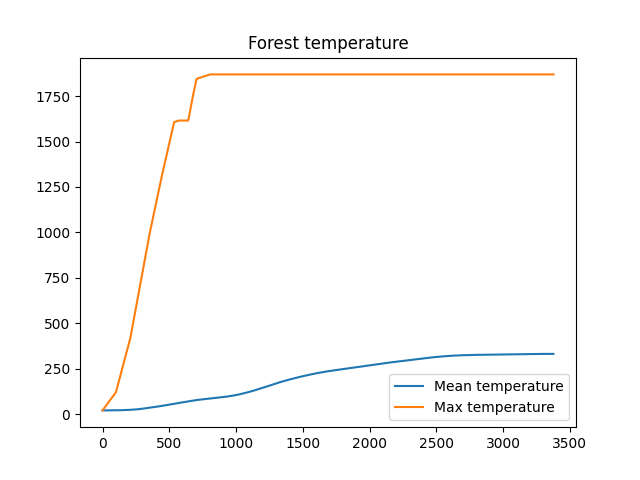
\includegraphics[width=\textwidth]{../src/runs/scenario1/temperature}
    \caption{Cenário 1 - Evolução da temperatura média e máxima}
    \label{fig:S1Temp}
\end{figure}


\section{Cenário 2}\label{sec:scenario2}

O segundo cenário apresenta uma inclinação negativa do terreno, de \ang{-30}, com vento sudeste de intensidade $(-10, 15)$ \si{\meter\per\second}, ou seja, contra a propagação do incêndio.
O modelo terminou com 71.4\% da floresta ardida, após 3359 ticks, ou 388 árvores em termos absolutos - 206 carvalhos e 182 pinheiros.

Apesar das condições adversas, o fogo propagou-se rapidamente, à semelhança do que aconteceu em~\ref{sec:scenario1}.
Quando analisadas as curvas das Fig.~\ref{fig:S2ForestBurnt} e~\ref{fig:S2TreesBurnt}, torna-se evidente que o modelo teve uma evolução quase idêntica, porventura graças à alta probabilidade de propagação (40\%). Novamente, as fagulhas, apresentam uma evolução mais instável, evidente pela Fig.~\ref{fig:S2Sparks}, atingindo um pico de 16 fagulhas por tick por volta dos 1400 ticks.
Por fim, a temperatura média ficou-se igualmente pelos $\SI{330}{\degreeCelsius}$, já a temperatura máxima, atingida após 800 ticks (Fig.~\ref{fig:S2Temp}), foi à volta de $\SI{1870}{\degreeCelsius}$.

\begin{figure}[H]
    \centering
    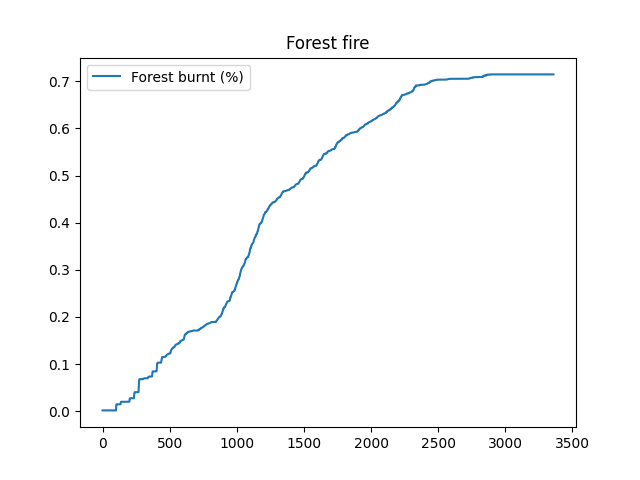
\includegraphics[width=\textwidth]{../src/runs/scenario2/forest_fire}
    \caption{Cenário 2 - Total de floresta ardida (em percentagem)}
    \label{fig:S2ForestBurnt}
\end{figure}

\begin{figure}[H]
    \centering
    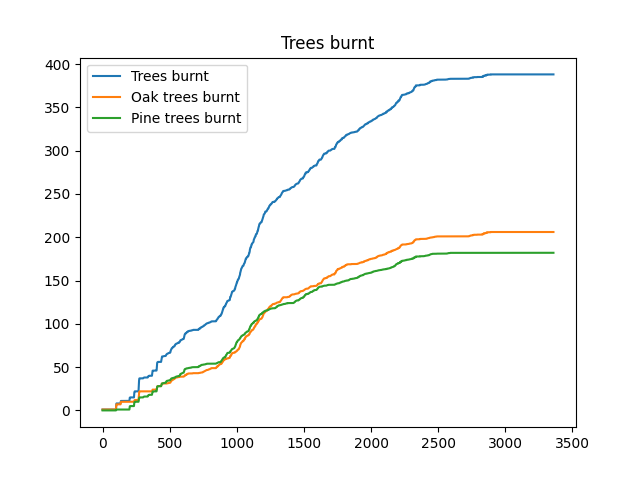
\includegraphics[width=\textwidth]{../src/runs/scenario2/trees_burnt}
    \caption{Cenário 2 - Total de árvores ardidas}
    \label{fig:S2TreesBurnt}
\end{figure}

\begin{figure}[H]
    \centering
    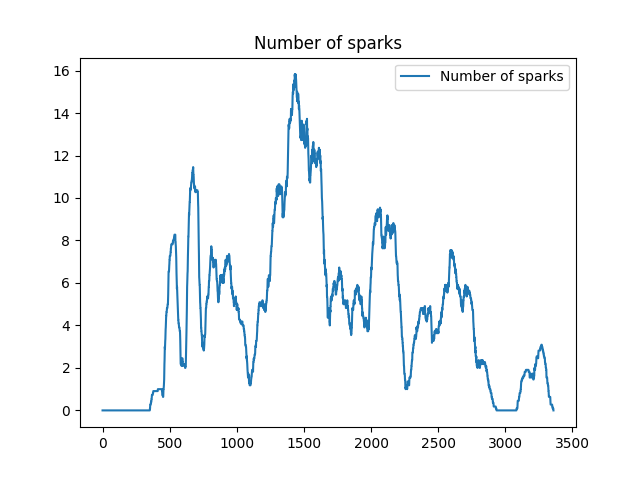
\includegraphics[width=\textwidth]{../src/runs/scenario2/sparks}
    \caption{Cenário 2 - Evolução do número de fagulhas}
    \label{fig:S2Sparks}
\end{figure}

\begin{figure}[H]
    \centering
    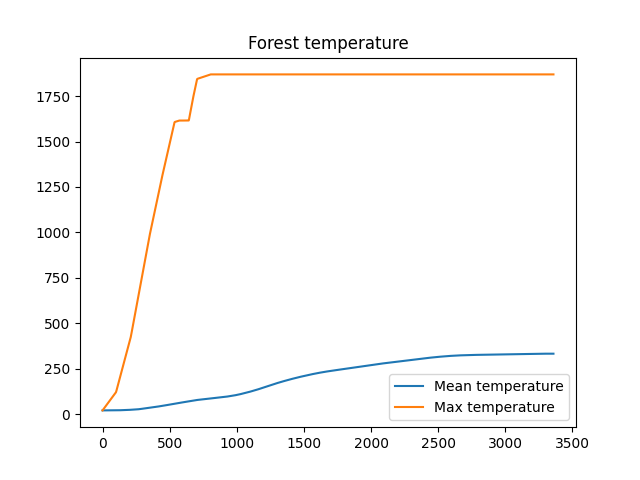
\includegraphics[width=\textwidth]{../src/runs/scenario2/temperature}
    \caption{Cenário 2 - Evolução da temperatura média e máxima}
    \label{fig:S2Temp}
\end{figure}


\section{Cenário 3}\label{sec:scenario3}

O terceiro cenário apresenta uma inclinação positiva do terreno, de \ang{30}, com vento noroeste de intensidade $(10, -15)$ \si{\meter\per\second}, ou seja, contra da propagação do incêndio.
O modelo terminou com 93.4\% da floresta ardida, após 3042 ticks, ou 508 árvores em termos absolutos - 250 carvalhos e 258 pinheiros.

O incêndio conseguiu destruir uma maior área da floresta, visível em Fig.~\ref{fig:S3ForestBurnt}, em menos tempo que os cenários anteriores.
Ao nível do tipo de árvores ardidas, dada a sua idêntica distribuição pelo terreno, não houve variações significativas entre pinheiros e carvalhos, como se pode constatar pela Fig.~\ref{fig:S3TreesBurnt}.
Também ao nível das fagulhas criadas, é possível notar um aumento considerável, com o modelo a atingir um pico de 18,5 fagulhas por tick por volta
1500 ticks (Fig.~\ref{fig:S3Sparks}). A temperatura média final foi ligeiramente superior, na ordem dos $\SI{412}{\degreeCelsius}$, já a temperatura máxima, atingida após 800 ticks (Fig.~\ref{fig:S3Temp}), manteve-se nos $\SI{1870}{\degreeCelsius}$.

\begin{figure}[H]
    \centering
    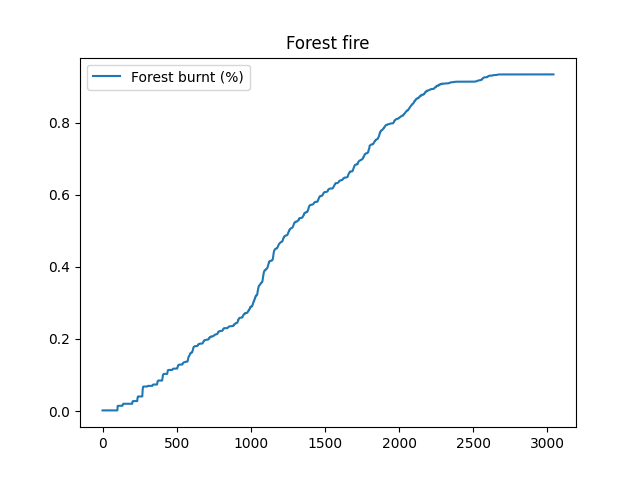
\includegraphics[width=\textwidth]{../src/runs/scenario3/forest_fire}
    \caption{Cenário 3 - Total de floresta ardida (em percentagem)}
    \label{fig:S3ForestBurnt}
\end{figure}

\begin{figure}[H]
    \centering
    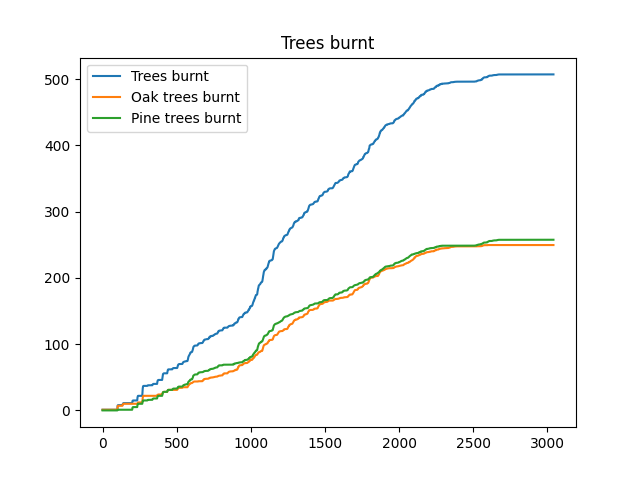
\includegraphics[width=\textwidth]{../src/runs/scenario3/trees_burnt}
    \caption{Cenário 3 - Total de árvores ardidas}
    \label{fig:S3TreesBurnt}
\end{figure}

\begin{figure}[H]
    \centering
    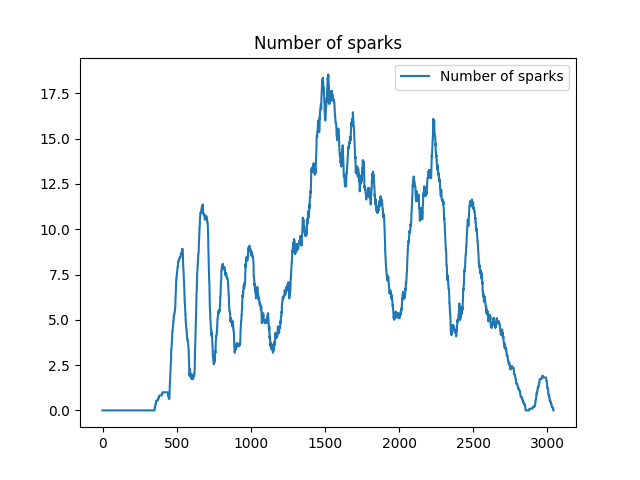
\includegraphics[width=\textwidth]{../src/runs/scenario3/sparks}
    \caption{Cenário 3 - Evolução do número de fagulhas}
    \label{fig:S3Sparks}
\end{figure}

\begin{figure}[H]
    \centering
    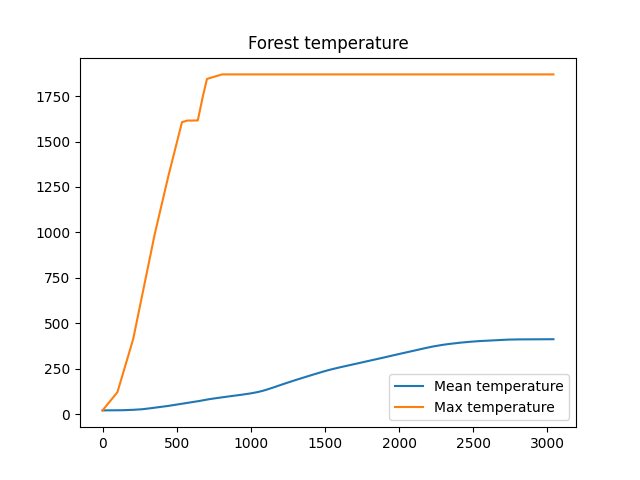
\includegraphics[width=\textwidth]{../src/runs/scenario3/temperature}
    \caption{Cenário 3 - Evolução da temperatura média e máxima}
    \label{fig:S3Temp}
\end{figure}


\section{Cenário 4}\label{sec:scenario4}

O quarto e último cenário apresenta uma inclinação negativa do terreno, de \ang{-30}, com vento noroeste de intensidade $(10, -15)$ \si{\meter\per\second}, ou seja, a favor da propagação do incêndio.
O modelo terminou com 93.3\% da floresta ardida, após 3103 ticks, ou 507 árvores em termos absolutos - 250 carvalhos e 257 pinheiros.

Este cenário apresenta condições de vento idênticas ao descrito em~\ref{sec:scenario3}, pelo que o modelo em si também evidenciou uma evolução do incêndio similar, quer ao nível da floresta ardida (Fig.~\ref{fig:S4ForestBurnt}), quer ao nível do tipo de árvores ardidas (Fig.~\ref{fig:S4TreesBurnt}).
No que concerne as fagulhas, o modelo atingiu um pico marginalmente superior, de 18,5 fagulhas por tick por volta 1500 ticks (Fig.~\ref{fig:S4Sparks}).
A temperatura média final foi por volta de $\SI{411}{\degreeCelsius}$, já a temperatura máxima, atingida após 800 ticks (Fig.~\ref{fig:S4Temp}), manteve-se nos $\SI{1870}{\degreeCelsius}$.

\begin{figure}[H]
    \centering
    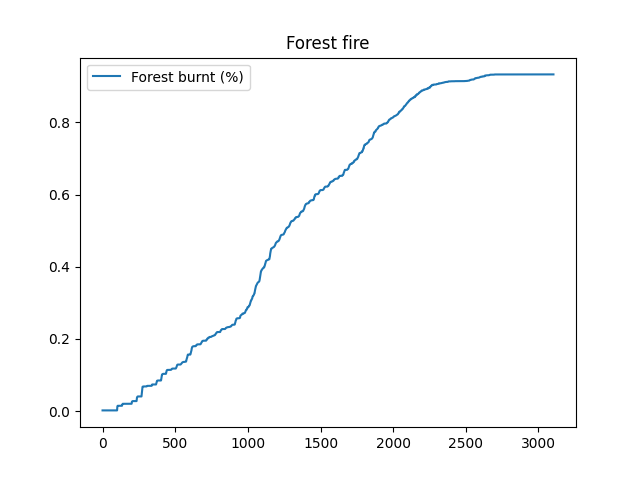
\includegraphics[width=\textwidth]{../src/runs/scenario4/forest_fire}
    \caption{Cenário 4 - Total de floresta ardida (em percentagem)}
    \label{fig:S4ForestBurnt}
\end{figure}

\begin{figure}[H]
    \centering
    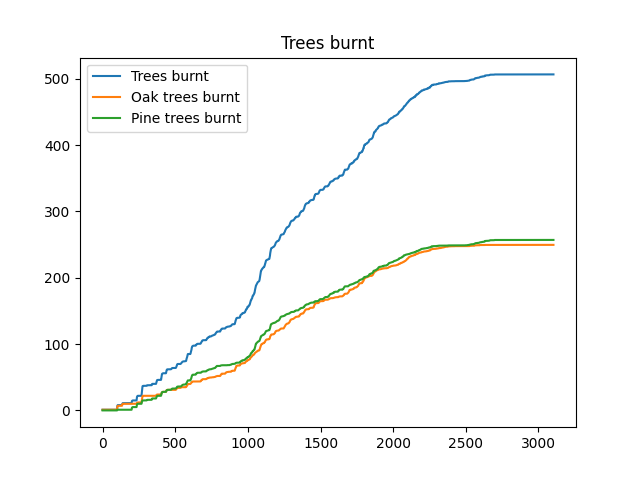
\includegraphics[width=\textwidth]{../src/runs/scenario4/trees_burnt}
    \caption{Cenário 4 - Total de árvores ardidas}
    \label{fig:S4TreesBurnt}
\end{figure}

\begin{figure}[H]
    \centering
    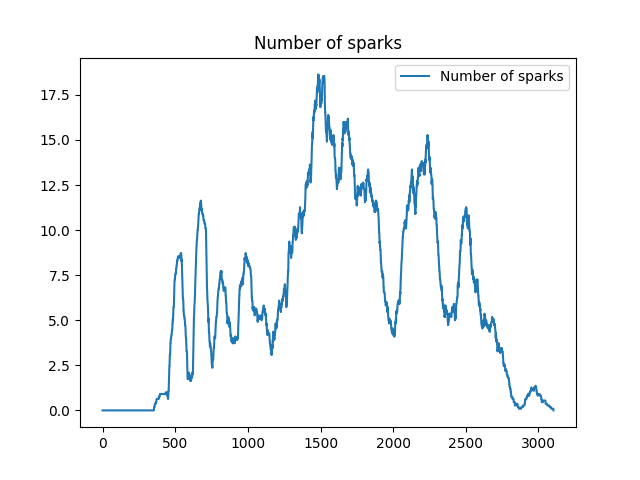
\includegraphics[width=\textwidth]{../src/runs/scenario4/sparks}
    \caption{Cenário 4 - Evolução do número de fagulhas}
    \label{fig:S4Sparks}
\end{figure}

\begin{figure}[H]
    \centering
    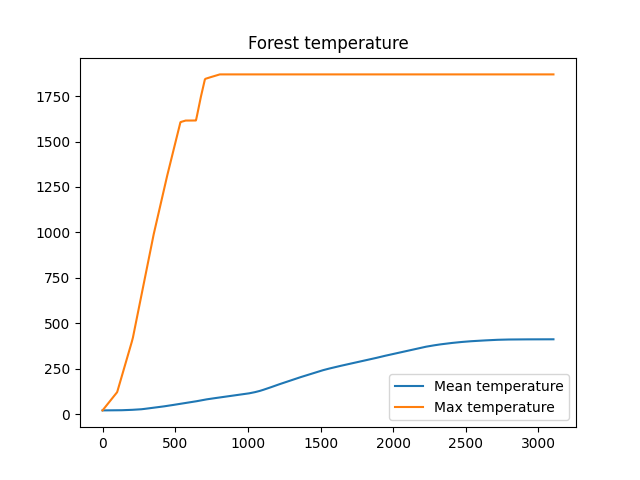
\includegraphics[width=\textwidth]{../src/runs/scenario4/temperature}
    \caption{Cenário 4 - Evolução da temperatura média e máxima}
    \label{fig:S4Temp}
\end{figure}